\documentclass[12pt,a4paper]{article}
\usepackage[utf8]{inputenc}
\usepackage[T1]{fontenc}
\usepackage[french]{babel}
\usepackage{amsmath}
\usepackage{graphicx}
\usepackage{hyperref}
\usepackage{booktabs}
\usepackage{float}
\usepackage{times} % Utilisation de la police Times New Roman


\hypersetup{
	colorlinks=true, % false: boxed links; true: colored links
	linkcolor=black, % color of internal links
	citecolor=black, % color of links to bibliography
	filecolor=black, % color of file links
	urlcolor=black   % color of external links
}

\title{Projet de l'UE Statistique avec SAS}
\author{Kossi Tonyi Wobubey ABOTSI}
\date{Université de Strasbourg (2023-2024)}

\begin{document}
	
	\maketitle
	
	\tableofcontents
	
	\newpage
	
	\section{Introduction}
	Ce projet, réalisé dans le cadre de l'unité d'enseignement "Statistiques avec SAS" au M1 Statistique, vise à appliquer les concepts statistiques à travers l'analyse de données réelles. Trois exercices explorent divers aspects de l'analyse statistique. Tous les tests statistiques effectués dans ce document sont réalisés avec un seuil \(\alpha = 5\%\).
	
	\section{Exercice I}
	
	\subsection{Énoncé}
	Nous disposons d'un échantillon de garçons et de filles provenant d'un district écossais. Cet échantillon est constitué d'observations indépendantes sur les caractéristiques de sexe et de couleur des cheveux, présentées dans un tableau.
	
	\textbf{Objectif :} Analyser la relation entre la couleur des cheveux et le sexe.
	
	\subsection{Visualisation des données et formulation d'une hypothèse}
	Les données sont présentées sous forme de tableau avec les caractéristiques de sexe et de couleur des cheveux.
	
	\begin{table}[H]
		\centering
		\begin{tabular}{@{}lccccc@{}}
			\toprule
			& \textbf{BLOND} & \textbf{ROUX} & \textbf{CHÂTAIN} & \textbf{BRUN} & \textbf{NOIR DE JAIS} \\ \midrule
			GARÇON & 592            & 119           & 849              & 504           & 36                    \\
			FILLE  & 544            & 97            & 677              & 451           & 14                    \\ \bottomrule
		\end{tabular}
		\caption{Répartition des couleurs de cheveux par genre}
	\end{table}
	
	Nous observons sur le graphique à barres empilées la répartition par sexe et couleur de cheveux (cf. script pour le code).
	
	\begin{figure}[H]
		\centering
		\includegraphics[width=\textwidth]{barre_empilé.PNG}
		\caption{Barres empilées de la répartition par sexe et couleur de cheveux}
		\label{fig:barre_empile}
	\end{figure}
	
	Ce graphique montre que les garçons ont légèrement plus de cheveux châtains et noirs de jais que les filles. Nous voulons donc déterminer si cette différence observée est statistiquement significative.

	\subsection{Choix du test à réaliser}
	Nous analysons deux variables qualitatives observées sur un échantillon pour tester leur indépendance. Le test le plus adapté dans cette situation est le \textbf{G-test}.
	
	\textbf{Les hypothèses à tester sont :}
	\begin{itemize}
		\item H0 : Les variables sexe et couleur des cheveux sont indépendantes.
		\item H1 : Les variables sexe et couleur des cheveux ne sont pas indépendantes.
	\end{itemize}
	
	\subsection{Vérification des conditions d'application}
	\subsubsection{Indépendance}
	Les observations dans le tableau de contingence ont été collectées de manière indépendante.
	\subsubsection{Exclusivité des classes}
	Chaque individu observé est classé dans une et une seule catégorie pour chacune des deux variables.
	\subsubsection{Règle de Cochran}
	Pour respecter cette règle, au moins 80\% des effectifs théoriques doivent être au moins égaux à 5.
	
	Voici le tableau des effectifs théoriques obtenus :
	
	\begin{table}[H]
		\centering
		\begin{tabular}{@{}lccccc@{}}
			\toprule
			& \textbf{BLOND}    & \textbf{ROUX}   & \textbf{CHÂTAIN} & \textbf{BRUN}   & \textbf{NOIR DE JAIS} \\ \midrule
			GARÇON & 614,37033         & 116,81689       & 825,28972        & 516,48210       & 27,04094              \\
			FILLE  & 521,62966         & 99,18310        & 700,71027        & 438,51789       & 22,95905              \\ \bottomrule
		\end{tabular}
		\caption{Répartition des couleurs de cheveux par genre avec valeurs décimales}
	\end{table}
	
	Nous observons dans le tableau ci-dessus que plus de 80\% des effectifs sont supérieurs à 5.
	
	Toutes les conditions d'application étant vérifiées, nous pouvons procéder au G-test (cf. script SAS). Nous obtenons une statistique \(\chi^2_{\text{obs}} = 10.7555\) qui, sous H0, suit une distribution \(\chi_{4}^2\) avec 4 degrés de liberté. La P-valeur observée est de 0.0295.
	
	\subsection{Conclusion}
	La P-valeur étant inférieure à 5\%, nous rejetons H0. Par conséquent, les variables sexe et couleur de cheveux ne sont pas indépendantes, ce qui indique que la différence observée est statistiquement significative. Le V de Cramer nous donne 0.0519, inférieur à 0.1, donc l'intensité de cette liaison est très faible mais pas négligeable.

	
	\section{Exercice II}
	
	\subsection{Énoncé}
	Une entreprise pharmaceutique expérimente une nouvelle molécule censée faire baisser une mesure physiologique chez des patients porteurs d’une pathologie. Pour cela, 54 patients sans lien de parenté ont été recrutés. Chaque patient s’est vu attribuer soit la nouvelle molécule (traitement A) soit un placebo (traitement B). Les groupes ont été constitués de manière à ce que les distributions de l’âge et du sexe soient similaires dans les deux groupes. Les données sont contenues dans le fichier \texttt{molecule.csv}.
	
	Questions :
	
	1. Quelles sont les moyennes et écarts-types dans chacun des groupes ?
	
	2. Est-ce que la molécule testée est efficace ?
	
	\textbf{Objectif :} Tester l'efficacité de la nouvelle molécule.
	
	\subsection{Statistiques descriptives}
	Les statistiques descriptives de notre jeu de données, où les valeurs affichées correspondent à une mesure physiologique pour des patients porteurs d'une pathologie, sont les suivantes :
	
	\begin{table}[H]
		\centering
		\begin{tabular}{ccc}
			\toprule
			& Traitement A & Traitement B \\
			\midrule
			Nombre d'observations & 27 & 27 \\
			Moyenne & 78.836 & 65.751 \\
			Écart-type & 11.141 & 12.416 \\
			\bottomrule
		\end{tabular}
		\caption{Moyenne et Écart-type dans chacun des groupes}
		\label{tab:example}
	\end{table}
	
	On observe que en moyenne la mesure physiologique des patients ayant subi le traitement A est supérieure à celle des patients ayant reçu le traitement B. La question maintenant est de savoir si cette différence observée est significative.
	
	\subsection{Test statistique}
	Pour déterminer si la molécule testée est efficace, nous allons comparer les moyennes des mesures effectuées sur les deux groupes. Ayant seulement deux groupes et une variable quantitative, le test adéquat à réaliser est le test de \textbf{Student}.
	
	Les hypothèses à tester sont :
	\begin{itemize}
		\item H0 : La mesure moyenne des patients ayant reçu le traitement A est la même que celle des patients ayant reçu le traitement B (placebo).
		\item H1 : La mesure moyenne des patients ayant reçu le traitement A est différente de celle des patients ayant reçu le traitement B (placebo).
	\end{itemize}
	
	\subsection{Vérification des conditions d'application}
	
	\subsubsection{Indépendance}
	Selon le protocole de collecte des données, les patients sans lien de parenté ont été recrutés, ce qui permet de conclure que nos observations sont indépendantes.
	
	\subsubsection{Normalité}
	Soit $Y$ notre variable d'intérêt et $Y_1$, $Y_2$ respectivement les variables dans les échantillons de \textbf{Traitement A} et \textbf{Traitement B}. Nous allons procéder au test de \textbf{Shapiro-Wilk} sur nos deux échantillons.
	
	Les hypothèses à tester sont :
	\begin{itemize}
		\item H0 : L'échantillon est issu d'une population normalement distribuée.
		\item H1 : L'échantillon n'est pas issu d'une population normalement distribuée.
	\end{itemize}
	
	Nos deux échantillons sont composés d'observations indépendantes issues d'une variable d'intérêt qui est quantitative continue. La condition d'application du test de \textbf{Shapiro-Wilk} est donc vérifiée.
	
	\textbf{Normalité de $Y_1$} : En procédant au test (cf. script), on obtient une p-valeur de \textbf{0.8149}. La p-valeur observée est supérieure au seuil $\alpha$, donc nous conservons l'hypothèse nulle H0. L'échantillon est issu d'une population normalement distribuée.
	
	\textbf{Normalité de $Y_2$} : En procédant au test (cf. script), on obtient une p-valeur de \textbf{0.9158}. La p-valeur observée est supérieure au seuil $\alpha$, donc nous conservons l'hypothèse nulle H0. L'échantillon est issu d'une population normalement distribuée.
	
	\subsubsection{Égalité des variances}
	Nous allons vérifier l'égalité des variances dans nos deux échantillons. Soit $\sigma_{1}^2$ et $\sigma_{2}^2$ les variances respectives inconnues des échantillons \textbf{Traitement A} et \textbf{Traitement B}. Pour ce faire, nous allons procéder au test de \textbf{Fisher-Snedecor}. Les hypothèses sont :
	\begin{itemize}
		\item H0 : $\sigma_{1}^2 = \sigma_{2}^2$
		\item H1 : $\sigma_{1}^2 \neq \sigma_{2}^2$
	\end{itemize}
	
	Les conditions d'application sont :
	\begin{itemize}
		\item Chaque échantillon est composé d'observations indépendantes.
		\item Les deux échantillons sont indépendants.
		\item $Y_1 \sim \mathcal{N}(\mu_1, \sigma_1^2)$
		\item $Y_2 \sim \mathcal{N}(\mu_2, \sigma_2^2)$
	\end{itemize}
	
	Les deux premières conditions sont déjà vérifiées, et les deux dernières sont vérifiées par les tests de normalité précédents. En procédant au test (cf. script), on obtient :
	La statistique de décision \textbf{F = 1.24}, qui sous H0 suit une loi de Fisher à 26 et 26 degrés de liberté. La p-valeur est de \textbf{0.5846}. La p-valeur est supérieure au seuil $\alpha$, donc nous conservons H0 : il y a égalité des variances.
	
	\subsection{Conclusion}
	Toutes les conditions d'application du test de Student sont vérifiées. Nous réalisons donc le test (cf. script). Nous observons une statistique \textbf{T = 4.08}, qui sous H0 suit la loi de Student à 52 degrés de liberté. La p-valeur est de \textbf{0.0002}. La p-valeur étant inférieure au seuil $\alpha$, nous rejetons H0. Donc, la moyenne des mesures effectuées dans les deux groupes est différente. On observe aussi que la moyenne de la mesure du groupe ayant eu le traitement A est supérieure à celle ayant eu le traitement B, ce qui indique que la molécule testée est inefficace puisqu'elle était censée faire baisser la mesure physiologique. Elle a plutôt un effet inverse.
	
\section{Exercice III}

\subsection{Énoncé}
La pollution de l’air constitue actuellement une des préoccupations majeures de santé publique. De nombreuses études épidémiologiques ont permis de mettre en évidence l’influence sur la santé de certains composés chimiques comme l’ozone (O3). Le jeu de données \texttt{ozone.xls} comporte 112 observations indépendantes relevées durant l’été 2001.

\begin{itemize}
	\item La variable maxO3 est le maximum journalier de la concentration en ozone (en $\mu g/m^3$).
	\item Les variables T9, T12, T15 correspondent aux températures relevées respectivement à 9h, 12h et 15h.
	\item Les variables Ne9, Ne12, Ne15 correspondent aux nébulosités relevées respectivement à 9h, 12h et 15h.
	\item Les variables Vx9, Vx12, Vx15 correspondent à la composante Est-Ouest du vent relevée respectivement à 9h, 12h et 15h.
\end{itemize}

Le but de l’exercice est d’étudier l’éventuelle relation linéaire entre la variable maxO3 et l’ensemble des autres variables. Pour cela, à l’aide de SAS, après avoir présenté les statistiques descriptives des variables, il faut appliquer un protocole de sélection du modèle. Le critère de sélection utilisé devra être présenté. Une fois le modèle optimal trouvé, il est demandé d’interpréter les résultats.

\textbf{Objectif :} Étudier la relation linéaire entre la variable maxO3 et l'ensemble des autres variables.

\subsection{Statistique descriptive}
\subsubsection{Tableau résumant les statistiques descriptives}
(cf. script pour le code)

\begin{table}[H]
	\centering
	\resizebox{\textwidth}{!}{
		\begin{tabular}{|l|r|r|r|r|r|r|r|r|r|}
			\hline
			\textbf{Variable} & \textbf{N} & \textbf{Nbre manquant} & \textbf{Moyenne} & \textbf{Écart-type} & \textbf{Min} & \textbf{1er Quartile} & \textbf{Médiane} & \textbf{3ème Quartile} & \textbf{Max} \\
			\hline
			maxO3 & 112 & 0 & 90.3035714 & 28.1872245 & 42 & 70.5 & 81.5 & 106 & 166 \\
			T9 & 112 & 0 & 18.3607143 & 3.1227257 & 11.3 & 16.2 & 17.8 & 19.95 & 27 \\
			T12 & 112 & 0 & 21.5267857 & 4.0423208 & 14 & 18.6 & 20.55 & 23.6 & 33.5 \\
			T15 & 112 & 0 & 22.6276786 & 4.5308594 & 14.9 & 19.25 & 22.05 & 25.6 & 35.5 \\
			Ne9 & 112 & 0 & 4.9285714 & 2.5949163 & 0 & 3 & 6 & 7 & 8 \\
			Ne12 & 112 & 0 & 5.0178571 & 2.2818601 & 0 & 4 & 5 & 7 & 8 \\
			Ne15 & 112 & 0 & 4.8303571 & 2.3322587 & 0 & 3 & 5 & 7 & 8 \\
			Vx9 & 112 & 0 & -1.2143455 & 2.6327423 & -7.8785 & -3.339 & -0.866 & 0.6946 & 5.1962 \\
			Vx12 & 112 & 0 & -1.6110036 & 2.7956729 & -7.8785 & -3.6294 & -1.8794 & 0 & 6.5778 \\
			Vx15 & 112 & 0 & -1.690683 & 2.8101977 & -9 & -3.9392 & -1.54965 & 0 & 5 \\
			\hline
		\end{tabular}
	}
	\caption{Statistiques descriptives}
\end{table}

\subsubsection{Visualisation des données}
Observons les nuages de points par paires (cf. script pour le code).

\begin{figure}[H]
	\centering
	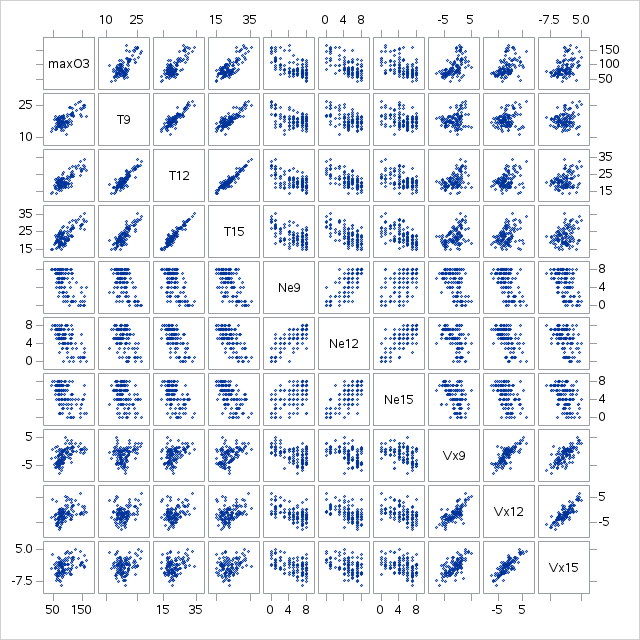
\includegraphics[width=\textwidth]{Nuage_de_point.png}
	\caption{Nuage de points}
	\label{fig:nuage_de_points}
\end{figure}

Comme on peut le voir ci-dessus, on remarque une relation linéaire (forte corrélation) entre les variables T9, T12, T15 et entre les variables Vx9, Vx12, Vx15.

\subsection{Modélisation}
Nous allons étudier la régression de la variable maxO3 par les variables T9, T12, T15, Ne9, Ne12, Ne15, Vx9, Vx12, Vx15 dans le cadre d'un modèle linéaire généralisé (GLM) de Poisson.

La variable maxO3 est supposée suivre une loi de Poisson de paramètre $\lambda$ car discrète et positive. Nos observations étant indépendantes grâce au protocole de collecte des données, nous utiliserons un GLM de Poisson pour étudier la relation linéaire entre maxO3 et les variables explicatives. La fonction de lien pour ce modèle est la fonction log.

Soit $Y = \text{maxO3}$. Nous avons donc $log(E(Y_i)) = \eta_i$, avec $\eta_i$ une combinaison linéaire des variables explicatives (T9, T12, T15, Ne9, Ne12, Ne15, Vx9, Vx12, Vx15), combinaison dont nous cherchons les coefficients, plus un coefficient constant.

Tous les résultats présentés ont leurs codes dans le script SAS.

Voici un extrait de la sortie liée à notre modèle :

\begin{figure}[H]
	\centering
	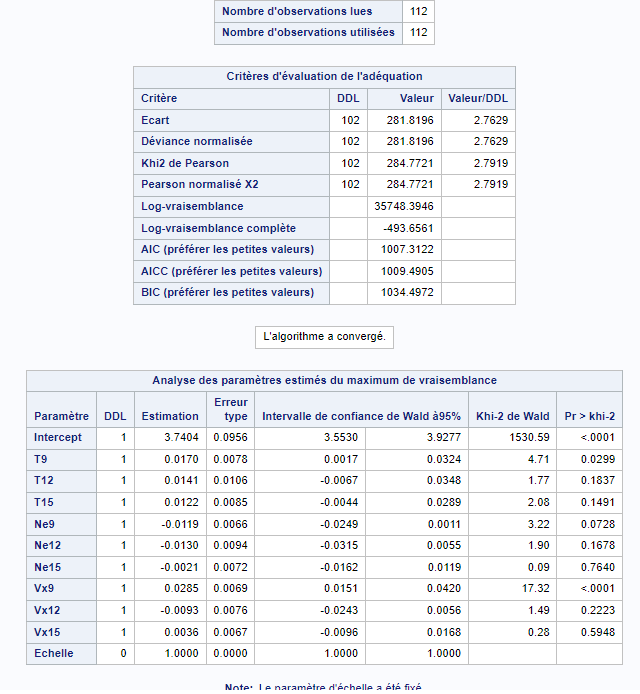
\includegraphics[width=\textwidth]{Sortie_GLM.PNG}
	\caption{Résultats du GLM de Poisson}
	\label{fig:resultats_glm_poisson}
\end{figure}

Ci-dessus nous avons l'estimation des paramètres du modèle et les tests de validité de ces paramètres.
Soit $\beta_j$ un paramètre du modèle sauf la constante. Les hypothèses du test de validité de ce paramètre sont :

\begin{itemize}
	\item H0 : $\beta_j = 0$
	\item H1 : $\beta_j \neq 0$
\end{itemize}

On utilise la statistique de test Q = $\hat{\beta_j}^2/\hat{\sigma_j}^2$ qui, sous H0, suit une loi du $\chi^2$ à 1 ddl.
Pour un niveau $\alpha=5\%$, on acceptera la nullité des paramètres associés aux variables T12, T15, Ne9, Ne12, Ne15, Vx12 et Vx15 car leurs p-valeurs observées sont supérieures à 5\% et on rejettera la nullité des paramètres associés aux variables T9 et Vx9 car leurs p-valeurs sont inférieures à 5\%.

\subsubsection{Élimination de l'information redondante dans notre modèle}
Nous allons étudier la corrélation entre les variables explicatives. Avant de procéder à la sélection de modèle, il est crucial de retirer toute redondance parmi les variables explicatives. Idéalement, ces variables devraient être indépendantes les unes des autres pour éviter des problèmes de multicolinéarité. Afin d'identifier et d'éliminer toute corrélation excessive entre elles, l'utilisation du Variance Inflation Factor (VIF) est recommandée. Un seuil de VIF = 10 est utilisé car notre modèle n'a pas de problème de sur-paramétrage, avec 112 observations pour au plus 10 paramètres.

On obtient le résultat suivant :

\begin{table}[H]
	\centering
	\begin{tabular}{|l|r|}
		\hline
		\textbf{Variable} & \textbf{VIF} \\
		\hline
		Intercept & 0 \\
		T9 & 6.02420 \\
		T12 & 17.99033 \\
		T15 & 14.44099 \\
		Ne9 & 3.08475 \\
		Ne12 & 5.18893 \\
		Ne15 & 2.93896 \\
		Vx9 & 2.94865 \\
		Vx12 & 4.65468 \\
		Vx15 & 3.56281 \\
		\hline
	\end{tabular}
	\caption{Variables et VIF correspondants}
\end{table}

On remarque que le VIF des variables explicatives T12 et T15 est supérieur à 10. Nous éliminons donc celle ayant le plus grand VIF, T12, et répétons l'analyse. On obtient :

\begin{table}[H]
	\centering
	\begin{tabular}{|l|r|}
		\hline
		\textbf{Variable} & \textbf{VIF} \\
		\hline
		Intercept & 0 \\
		T9 & 4.57296 \\
		T15 & 6.73019 \\
		Ne9 & 3.03129 \\
		Ne12 & 3.99759 \\
		Ne15 & 2.43735 \\
		Vx9 & 2.85535 \\
		Vx12 & 4.47157 \\
		Vx15 & 3.51988 \\
		\hline
	\end{tabular}
	\caption{Variables et VIF correspondants après élimination}
\end{table}

Tous les VIF sont maintenant inférieurs à 10. Nous avons donc notre modèle optimal au sens du VIF, c'est-à-dire que les variables explicatives ne sont pas trop corrélées.

\subsubsection{Vérification de la surdispersion dans notre modèle}
La variable maxO3 modélisée par une loi de Poisson mais la variance n'est pas forcément égale à l'espérance. Dans notre cas, la variance est $\phi \times \text{espérance}$, l'idéal étant que $\phi = 1$ avec $\phi = \text{déviance}/(n - p)$, où $p$ est le nombre de paramètres et $n$ l'effectif de l'échantillon. Or, on observe $\phi = 2.7629$, supérieur à 1, ce qui indique une surdispersion.

Pour corriger ce problème, nous introduisons un paramètre dans le modèle permettant de ramener $\phi$ à 1. Le code incluant la correction se trouve dans le script SAS. Nous effectuons ensuite la sélection de modèle avec cette correction.

\subsubsection{Sélection de modèle}
Nous allons maintenant entreprendre la sélection du modèle. Notre modèle n'a pas de problème de surparamétrage. L'idéal serait de faire une sélection de modèle à l'aide de l'AIC avec la méthode du backward. Cependant, avec la correction effectuée due à la surdispersion, nous ne pouvons plus calculer la vraisemblance car la loi n'est plus Poisson mais quasi-Poisson. Donc le choix qui s'offre à nous est les tests LRT.

\textbf{Hypothèses :}
\begin{itemize}
	\item H0 : Il n'y a pas de différence significative entre M1 et M2 (M1 : modèle complet, M2 : modèle avec une variable de moins)
	\item H1 : Il y a une différence significative entre M1 et M2
\end{itemize}

En effectuant le test, voici le premier résultat :

\begin{figure}[H]
	\centering
	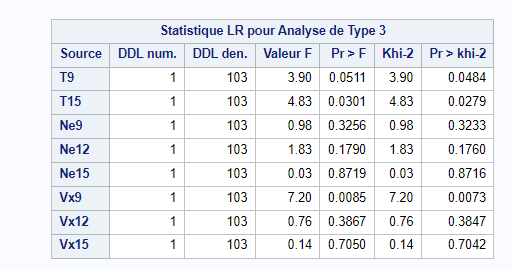
\includegraphics[width=\textwidth]{LRT_1.PNG}
	\caption{Résultats du test LRT}
	\label{fig:resultats_lrt1}
\end{figure}

La variable Ne15 a une p-valeur de \textbf{0.8716}, la plus grande, supérieure au seuil de 5\%, donc si elle est éliminée du modèle, il n'y a aucune différence significative avec l'ancien modèle.

Effectuons de nouveau le test sans la variable Ne15, on obtient :

\begin{figure}[H]
	\centering
	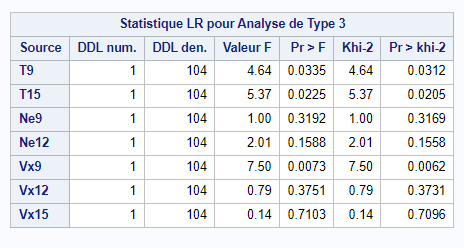
\includegraphics[width=\textwidth]{LRT_2.PNG}
	\caption{Résultats du test LRT}
	\label{fig:resultats_lrt2}
\end{figure}

La variable Vx15 a une p-valeur de \textbf{0.7096}, la plus grande, supérieure au seuil de 5\%, donc si elle est éliminée du modèle, il n'y a aucune différence significative avec l'ancien modèle.

Effectuons de nouveau le test sans la variable Vx15, on obtient :

\begin{figure}[H]
	\centering
	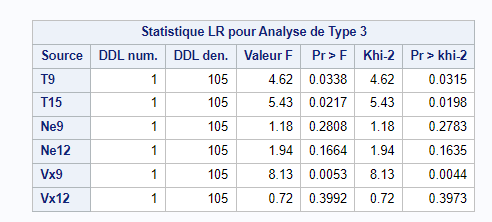
\includegraphics[width=\textwidth]{LRT_3.PNG}
	\caption{Résultats du test LRT}
	\label{fig:resultats_lrt3}
\end{figure}

La variable Vx12 a une p-valeur de \textbf{0.3973}, la plus grande, supérieure au seuil de 5\%, donc si elle est éliminée du modèle, il n'y a aucune différence significative avec l'ancien modèle.

Effectuons de nouveau le test sans la variable Vx12, on obtient :

\begin{figure}[H]
	\centering
	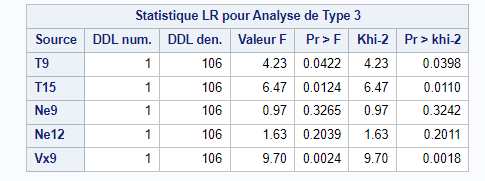
\includegraphics[width=\textwidth]{LRT_4.PNG}
	\caption{Résultats du test LRT}
	\label{fig:resultats_lrt4}
\end{figure}

La variable Ne9 a une p-valeur de \textbf{0.3242}, la plus grande, supérieure au seuil de 5\%, donc si elle est éliminée du modèle, il n'y a aucune différence significative avec l'ancien modèle.

Effectuons de nouveau le test sans la variable Ne9, on obtient :

\begin{figure}[H]
	\centering
	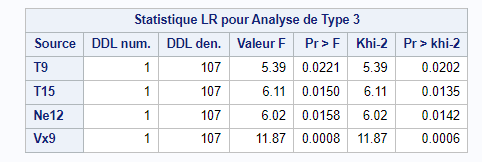
\includegraphics[width=\textwidth]{LRT_5.PNG}
	\caption{Résultats du test LRT}
	\label{fig:resultats_lrt5}
\end{figure}

Toutes les variables (T9, T15, Ne12, Vx9) ont une p-valeur inférieure au seuil de 5\%, donc si l'une d'entre elles est éliminée, il y aura une différence significative avec l'ancien modèle.

Voici le résumé du modèle final, le modèle optimal après la sélection de modèle :

\begin{figure}[H]
	\centering
	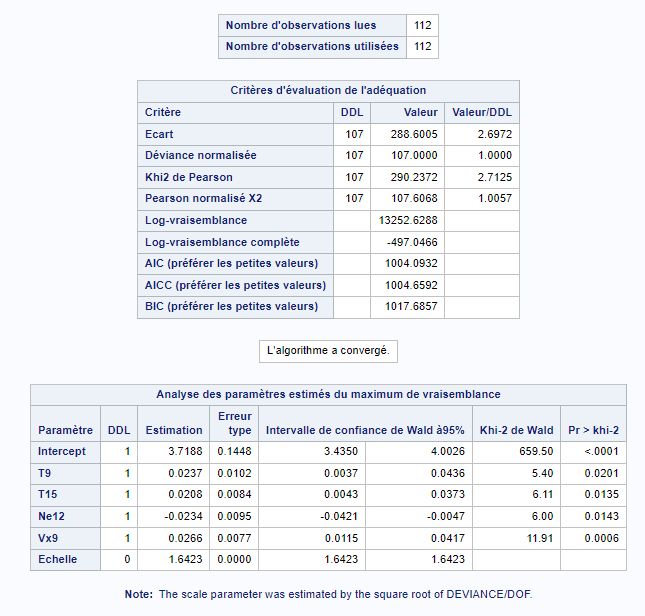
\includegraphics[width=\textwidth]{Model_Final_GLM.PNG}
	\caption{Modèle final}
	\label{fig:modele_final}
\end{figure}

\textbf{Interprétation :}

Tous les paramètres du modèle (Intercept, T9, T15, Ne12, Vx9) sont statistiquement significatifs, avec des p-valeurs inférieures à 0.05, ce qui signifie que chacun de ces paramètres a un effet significatif sur la variable de réponse dans le modèle de Poisson.

\begin{itemize}
	\item \textbf{Intercept}
	\begin{itemize}
		\item \textbf{Estimation} : 3.7188
		\item \textbf{Erreur type} : 0.1448
		\item \textbf{Intervalle de confiance de Wald à 95\%} : [3.4350, 4.0026]
		\item \textbf{Khi-2 de Wald} : 659.50
		\item \textbf{Pr > khi-2} : <0.0001
	\end{itemize}
	L'intercept représente le log du maxO3 lorsque toutes les variables indépendantes sont égales à zéro. Son estimation est très significative (p-valeur < 0.0001), indiquant qu'il y a un effet de base substantiel.
	
	\item \textbf{T9}
	\begin{itemize}
		\item \textbf{Estimation} : 0.0237
		\item \textbf{Erreur type} : 0.0102
		\item \textbf{Intervalle de confiance de Wald à 95\%} : [0.0037, 0.0436]
		\item \textbf{Khi-2 de Wald} : 5.45
		\item \textbf{Pr > khi-2} : 0.0195
	\end{itemize}
	La variable T9 a un coefficient positif et significatif (p-valeur = 0.0195). Cela signifie que pour chaque unité d'augmentation de T9, le log du maxO3 augmente de 0.0237, toute chose étant égale par ailleurs, ce qui correspond à une valeur de maxO3 multipliée par $\exp(0.0237) \approx 1.024$.
	
	\item \textbf{T15}
	\begin{itemize}
		\item \textbf{Estimation} : 0.0208
		\item \textbf{Erreur type} : 0.0084
		\item \textbf{Intervalle de confiance de Wald à 95\%} : [0.0043, 0.0373]
		\item \textbf{Khi-2 de Wald} : 6.16
		\item \textbf{Pr > khi-2} : 0.0131
	\end{itemize}
	La variable T15 a également un coefficient positif et significatif (p-valeur = 0.0131). Une augmentation d'une unité de T15 entraîne une augmentation du log du maxO3 de 0.0208, toute chose étant égale par ailleurs, soit une valeur de maxO3 multipliée par $\exp(0.0208) \approx 1.021$.
	
	\item \textbf{Ne12}
	\begin{itemize}
		\item \textbf{Estimation} : -0.0234
		\item \textbf{Erreur type} : 0.0095
		\item \textbf{Intervalle de confiance de Wald à 95\%} : [-0.0420, -0.0047]
		\item \textbf{Khi-2 de Wald} : 6.02
		\item \textbf{Pr > khi-2} : 0.0142
	\end{itemize}
	La variable Ne12 a un coefficient négatif et significatif (p-valeur = 0.0142). Cela signifie qu'une augmentation d'une unité de Ne12 entraîne une diminution du log de maxO3 de 0.0234, toute chose étant égale par ailleurs, soit une valeur de maxO3 multipliée par $\exp(-0.0234) \approx 0.977$.
	
	\item \textbf{Vx9}
	\begin{itemize}
		\item \textbf{Estimation} : 0.0206
		\item \textbf{Erreur type} : 0.0077
		\item \textbf{Intervalle de confiance de Wald à 95\%} : [0.0115, 0.0297]
		\item \textbf{Khi-2 de Wald} : 11.91
		\item \textbf{Pr > khi-2} : 0.0006
	\end{itemize}
	La variable Vx9 a un coefficient positif et très significatif (p-valeur = 0.0006). Une augmentation d'une unité de Vx9 augmente le log du maxO3 de 0.0206, toute chose étant égale par ailleurs, soit une valeur de maxO3 multipliée par $\exp(0.0206) \approx 1.021$.
\end{itemize}

\subsection{Conclusion}
Les variables T9, T15, et Vx9 ont des effets positifs et significatifs sur la variable maxO3, tandis que Ne12 a un effet négatif et significatif. Ces résultats peuvent être utilisés pour comprendre les influences des différentes variables sur la variable dépendante, en tenant compte des effets multiplicatifs sur le taux d'incidence dans un cadre de modèle de Poisson.


\end{document}






